\section{\LangOO, The programming language }  

\subsection{\LangOO syntax runtime configurations}
\label{sub:Loo} 
\sdN{This work} is based
 \LangOO, a {small}, imperative, sequential,  class based, typed, object-oriented language. 
 \sdN{We believe, however, that the work can easily adapted to any capability safe language with some form of encapsulation. 
Wrt to encapsulation and  capability safety},  \LangOO supports private fields, private and public methods, unforgeable addresses, and no ambient authority (no static methods, no address manipulation).
 It has a simple concept of module with module-private fields and methods, described in Sect. \ref{sect:execution}.
 The definition of \LangOO  {can be found in the appendices  \cite{necessityFull}}, and is  similar to   OOPSLA-22.\footnoteSD{any differences?}

A \LangOO state, $\sigma$,  consists of a  heap $\chi$, and a   stack $\psi$. A stack is is a sequence of frames, $\phi$.
A frame consists of a local variable map, and a continuation, \ie a sequence of statements to be executed.


 
\paragraph{Notation} We adopt the following, unsurprising, notation:
\begin{itemize}
\item
{An object is uniquely identified by the address that points to it. We shall be talking of objects $o$, $o'$ when talking less formally, and of addresses, $\alpha$, $\alpha'$, $\alpha_1$, ...  when more formal.}
\item
$x$, $x'$,  ..., $y$, ... $z$, ... are variables;  $\va$, $\va'$ ... are either addresses or variables, we call these \emph{\atoms}.
\item
$\alpha \in \sigma$ means that $\alpha$ is defined in the heap of $\sigma$, and $x\in \sigma$ means that $x$ is defined in the top frame of $\sigma$.
Conversely,  $\alpha\notin\sigma$ and $x\notin\sigma$ %, and $\va \notin A$ h
 have the obvious meanings.
\item
$\interpret{\sigma}{\alpha}$  is $\alpha$; and $\interpret{\sigma}{x}$  is the value to which  $x$  is mapped in the top-most frame of $\sigma$'s stack, 
and $\interpret{\sigma}{e.f}$ looks up in $\sigma$'s heap the value of $f$ for the object  $\interpret{\sigma}{e}$.
Note that $\interpret{\sigma}{e}$ is not defined when $e$ contains a method call or a ghost field.
\item The substitution  $\sigma[x \mapsto \alpha]$ is applied to the top frame of $\sigma$, and $\sigma[\overline{x \mapsto \alpha}]$ % applies the substitutions $\overline{x \mapsto \alpha}$ to the top frame.
has the expected meaning.
\item
{$\phi.\prg{local\_map}$ is the local variable map of $\phi$}, and $\sigma.\prg{cont}$ is the continuation in the top frame.
\item
$text_1 \txteq text_2$ expresses that $text_1$ and $text_2$ are textually equal.
\end{itemize}

  

  
\subsection{\LangOO Execution}
\label{sect:execution}

%Central to our work is the distriction between the 
 \LangOO execution is described by a small steps operational semantics of the shape $\leadstoOrig  {\Mtwo} {\sigma}   {\sigma'}$.\\
  $\Mtwo$ stands for one or more modules, where a
  module,  $M$, maps class names to class definitions. 
   
{The semantics enforces dynamically a simple form of module-wide privacy: 
Fields may be read or written only if the class of the object whose field is being read or written, and the class of the object which is reading or writing belong to the same module.}
Private methods may be called only if the class of the receiver (the object whose method is being called), and the class of the caller (the object which is calling) belong to the same module.
Public methods may always be called.

The semantics is as unsurprising in all remaining aspects  :  
In $\sigma$, the  top frame's continuation contains the statement to be  executed next.  
 Statements may assign to variables, allocate new objects, 
perform field reads and writes on objects, and
 call methods on those objects. 
When a method is called, a new frame is pushed onto the stack; this frame  maps \prg{this} and the formal parameters to  the values for the receiver and other arguments, and the continuation to the body of the method.  When the continuation is ground\footnoteSD{TODO check and define}, the frame is popped and the value from the last frame's continuation is entered into the appropriate part in the caller's continuation. 
%In other aspects, the semantics is unsurprisring.%we return from that call, its frame is  popped, and execution continues in the context of the calling method. 
%The relation $\leadstoOrigStar  {\Mtwo} {\_}   {\_}$  is the reflexive, transitive closure of $\leadstoOrig  {\Mtwo} {\_}   {\_}$ .


{Fig. \ref{fig:UpSemantics} illustrates  such  execution steps:  disks indicate states;
 horizontal $\leadstoN$-arrows denote   steps  within the same  call; upwards arrows denote  method calls;
 %(pushing a new frame onto the stack);  
 downwards arrows denote method returns. % (popping the top of the stack). 
 Here,   $\leadstoOrig {\Mtwo}{\sigma_8}   {\sigma_9} $ is a step within the same call, $\leadstoOrig {\Mtwo}{\sigma_9}   {\sigma_{10}} $ is a method call   
with $\leadstoOrig {\Mtwo}{\sigma_{12}}   {\sigma_{13}} $ %is a method return  (from the call to $m_a$), 
the corresponding return. 
 {Note that  $\leadstoOrigStar  {\Mtwo} {\sigma}   {\sigma'}$ may involve  any number of  calls or returns: 
 $\leadstoOrigStar  {\Mtwo} {\sigma_8}   {\sigma_{12}}$ involves one call and no return,
while $\leadstoOrigStar  {\Mtwo} {\sigma_{10}}   {\sigma_{15}}$,   involves no calls and two returns.
% In section \ref{sect:bounded}, we will define a derived relation, called bounded execution, where the number of returns may not exceed the number of calls.
}
} 

\begin{figure}[htb]
\begin{tabular}{|c|}
 \hline %  \\ -- this added one vertical space
\resizebox{7cm}{!}{
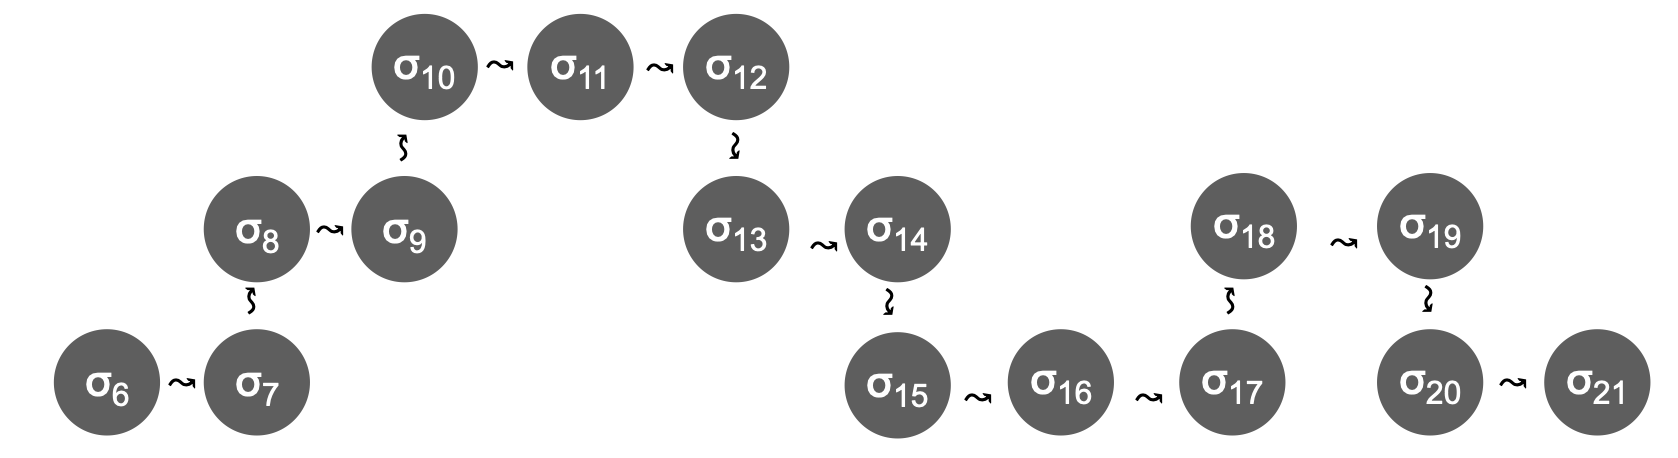
\includegraphics[width=\linewidth]{diagrams/bounded.png}
} 
 \\
\hline
%\begin{tabular}{lclclclcl}
%$\leadstoOrig  {\Mtwo} {\sigma_8}    {\sigma_9} $  & & 
%$\leadstoOrig  {\Mtwo} {\sigma_9}    {\sigma_{10}} $ &  &
%$\leadstoOrig  {\Mtwo} {\sigma_{12}}   {\sigma_{13}} $ & & 
%$\leadstoOrig  {\Mtwo} {\sigma_{13}}    {\sigma_{14}} $  &  &
%$\leadstoOrig {\Mtwo}{\sigma_{14}}   {\sigma_{15}} $
%\\
%\hline
%$\leadstoOrigStar  {\Mtwo} {\sigma_8}   {\sigma_{12}}$ & & \ & & \ & & $\leadstoOrigStar  {\Mtwo} {\sigma_{10}}   {\sigma_{15}}$
%\\
%\hline
%\end{tabular}
%\\
%\hline
\end{tabular}
   \caption{Illustrating   $\leadstoOrig  {\Mtwo} {\sigma}    {\sigma'}$ 
    }
   \label{fig:UpSemantics}
 \end{figure}
 
%\susan{I don't think the two lines at the bottom of the figure are needed here and in the next figure. {agree, but highlight.}} 
 
%{Note that $\leadstoOrig {\Mtwo}{\sigma_{8}}   {\sigma_{9}} $ and $\leadstoOrig {\Mtwo}{\sigma_{13}}   {\sigma_{14}} $ are steps within the same call, but 
%$\leadstoOrig {\Mtwo}{\sigma_{14}}   {\sigma_{15}} $ and $\leadstoOrig {\Mtwo}{\sigma_{17}}   {\sigma_{18}} $ are not. %steps within the same call,
%% even though all four states ($\sigma_{13}$, $\sigma_{14}$, $\sigma_{17}$, and $\sigma_{18}$), have the same number of frames on their stack.
%We want a semantics to reflect whether execution steps happen within the bounds of certain call. For this, we define \emph{bounded execution}, 
%$\leadstoBounded {\Mtwo} {\sigma} {\sigma''} {\sigma'}$ 
%which are execution steps which lead from $\sigma$ to $\sigma'$ while not popping  $\sigma''$-s top frame.
%This will be defined in Section \ref{sect:bounded}.
%}

\subsection*{Applicability} 
While our work is based on the particular language  \LangOO , % a simple, imperative, typed, object oriented  language with unforgeable addresses and private fields, we believe that % our approach
we believe that it is applicable to several programming paradigms, and  that   unforgeability and privacy
 can be replaced  by lower level mechanisms such as capability machines \cite{vanproving,davis2019cheriabi}.


\section{From \LangOO to \AssertLang}

{To develop the semantics of our assertions language, \AssertLang, we   build three auxiliary concepts on  top of  \LangOO: bounded execution, method calls and returns, and reachable objects.}


\subsection{Bounded Execution}
\label{sect:bounded}

{The semantics from the earlier section allows arbitrary numbers of method calls and returns. 
In particular, it is possible to start with a state $\sigma$ and perform more returns than calls --
\eg $\leadstoOrigStar  {\Mtwo} {\sigma_{8}}   {\sigma_{15}}$  in  Fig. \ref{fig:UpSemantics}.
{In the sense of $\leadsto^*$,  the state $\sigma_{15}$  is one of the future'states for $\sigma_8$.}

% This  is  is a perfectly natural semantics,  but
{For} the purposes of our work, we {also} need an {additional} notion, of    \emph{bounded} future state, which  can be reached through any  \red{number of} steps, including method calls and returns, but \red{stopping before returning} %excluding returns 
from the currently executing method} -- \cf Def. \ref{def:necessity-semantics}(2). 
\kjx{FWIW, I bet this does resolve to ``domination'' in a call graph
  (rather than a sequence of states)\red{SD: That would be right if the call graph had edges back from the callee to the caller. But our semantics does not have that, and I do not know of any small steps semantics that has this. AALSO: Can you comment please on whether you understand the definition  as written here?}}
Thus, the {bounded} future states of $\sigma_8$  only include 
 % states which are being visited as a result of  executing $\sigma_8$'s top continuation}; that is, it includes the states 
 $\sigma_9$, $\sigma_{10}$, $\sigma_{11}$, $\sigma_{12}$, $\sigma_{13}$, and $\sigma_{14}$, but \emph{not} $\sigma_{15}$  -- the latter results from returning from $\sigma_{8}$'s top continuation.  
 {Similarly, $\sigma_{18}$ is not a bounded future state of $\sigma_8$, even though they have the same stack depth -- between $\sigma_{8}$ 
 and  $\sigma_{18}$ we returned from the top continuation in $\sigma_{8}$.}
% since $\sigma$'s top frame will have been popped before we reach $\sigma'$. 

\newcommand{\bd}{_{bd}}

To obtain this  notion of {bounded} future, we define  \emph{execution} % from the viewpoint of an original state, 
{\emph{bounded by a state} $\sigma\bd$, which %  is ``bounded'' so as not to ever 
allows any steps, except for popping   $\sigma\bd$'s top frame:}
 
 
\begin{definition}[Bounded Execution]
\label{def:shallow:term}
We define relations \    $\leadstoBoundedThree {\Mtwo} {\sigma} {\sigma\bd} {\sigma'}$ \ and\  $\leadstoBounded  {\Mtwo} {\sigma} {\sigma'}$ as:

\begin{itemize}
\item
 $\leadstoBoundedThree {\Mtwo} {\sigma} {\sigma\bd}  {\sigma'}$ \    iff \ \   $\leadstoOrig {\Mtwo} {\sigma} {\sigma'} % $\\
% $\strut  \hspace{3.6cm}\ 
\ \  \wedge $\\
$\strut  \hspace{2.9cm}\ \      \exists \phi,\!\psi,\!\psi_1,\!\psi_2.[ \  \sigma\bd\! =\! (\phi\cdot\psi,\_) \ \wedge \ \sigma\! =\! (\psi_1\cdot \psi, \_)
\ \wedge\ \sigma'\! =\! (\psi_2\cdot \psi, \_)\ \wedge\ {\psi_1,\psi_2\!\neq\! \epsilon}] $ 
\item
 $\leadstoBoundedStarThree  {\Mtwo}  {\sigma}  {\sigma\bd} {\sigma'}$\ \  iff \ \ $\sigma=\sigma'\ \ \vee$\\
$\strut  \hspace{3cm}\ \ \exists n\!\in\!\mathbb{N},\sigma_0,..,\sigma_n.[\ \forall i\!\! \in\!\! [0..n).\leadstoBoundedThree {\Mtwo}  {\sigma_i}  {\sigma\bd} {\sigma_{i+1}} \ \wedge\ \sigma=\sigma_0\ \wedge\ \sigma'=\sigma_n\ ]$
 \item
{  $\leadstoBounded  {\Mtwo} {\sigma}   {\sigma'}$\ \  \ \ \ \ \ \   \ \ \ \ iff \ \ \ $\leadstoBoundedThree {\Mtwo} {\sigma} {\sigma}  {\sigma'}$}
  \item
{  $\leadstoBoundedStar {\Mtwo}  {\sigma}  {\sigma'}  $\ \ \ \ \ \ \ \ \   \ iff \ \ \ $\leadstoBoundedStarThree {\Mtwo}  {\sigma}  {\sigma} {\sigma'}$}\ \  
\item
\red{  $\leadstoBoundedStarFin {\Mtwo}  {\sigma}  {\sigma'}  $\ \ \ \ \ \   \ iff \ \ \ $\leadstoBoundedStar {\Mtwo}  {\sigma}  {\sigma'}  \ \wedge\ \ \neg(\exists 
\sigma''.[\  \leadstoBoundedThree {\Mtwo} {\sigma'}  {\sigma} {\sigma''} \ ]$ }
 \end{itemize}
\end{definition}
 

We continue with  Fig. \ref{fig:UpSemantics}. Here $\leadstoOrig {\Mtwo} {\sigma_{14}}  {\sigma_{15}}$ 
 but    $\notLeadstoBoundedThree {\Mtwo}  {\sigma_{14}} {\sigma_{14}} {\sigma_{15}}$
and  $\notLeadstoBounded  {\Mtwo}  {\sigma_{14}}   {\sigma_{15}}$
--  this step would pop  $\sigma_{14}$'s
 top frame. 
% Therefore,   $\leadstoOrigStar {\Mtwo} {\sigma_8}  {\sigma_{15}}$ 
%  but  $\notLeadstoBoundedStarThree {\Mtwo} {\sigma_8} {\sigma_8} {\sigma_{15}}$, and  $\notLeadstoBoundedStarThree {\Mtwo}  {\sigma_8} {\sigma_{15}}$.
 Also, $\leadstoOrigStar {\Mtwo} {\sigma_8}  {\sigma_{18}}$ 
 but  $\notLeadstoBoundedStar {\Mtwo} {\sigma_8}   {\sigma_{18}}$  -- even though $\sigma_8$ and $\sigma_{18}$ have the same depth of stack, they belong to different calls.
  

 %\begin{figure}[htb]
%\begin{tabular}{|c|}
% \hline %  \\ -- this added one vertical space
%\resizebox{7cm}{!}{
%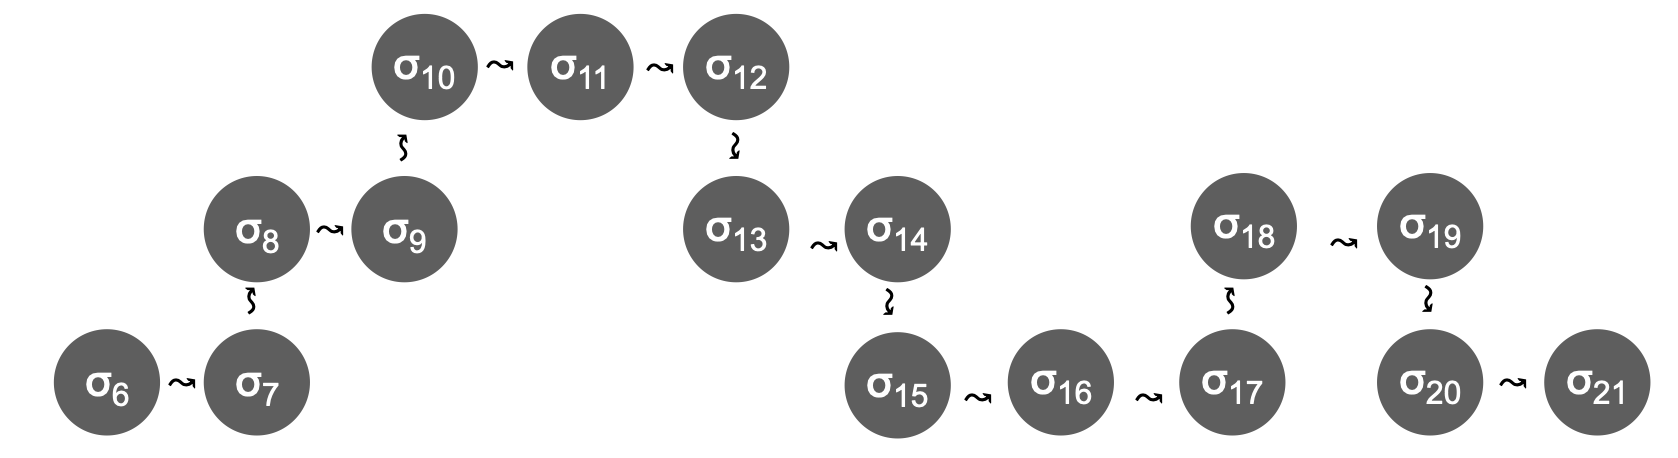
\includegraphics[width=\linewidth]{diagrams/bounded.png}
%} 
% \\
%\hline
%\begin{tabular}{lclclclclcl}
% $\leadstoBoundedThree  {\Mtwo} {\sigma_{12}} {\sigma_8}  {\sigma_{13}} $  & &   $\leadstoBoundedThree {\Mtwo} {\sigma_{13}}  {\sigma_{8}}  {\sigma_{14}} $ &  & \leadstoBoundedStar   {\Mtwo}   {\sigma_8}  {\sigma_{14}}  & &
%$\notLeadstoBoundedThree  {\Mtwo} {\sigma_{14}} {\sigma_8}  {\sigma_{15}} $ & &  
%\\
%\end{tabular}
%\\
%\hline
%\end{tabular}
%   \caption{Illustrating   $\leadstoBoundedThree  {\Mtwo} {\sigma}  {\sigma_o} {\sigma'}$, and $\leadstoBounded {\Mtwo} {\sigma}   {\sigma'}$}
%   \label{fig:UpSemanticsBounded}
% \end{figure}

%  \vspace{.1cm}
% \susan{you have removed an explanatory sentence that I found useful. It was the one that I wanted to put the word 'earlier' in}

Bounded semantics impose restrictions on the set of future states, but only from the viewpoint of {the bounding} \susan{binding?\red{SD: I thought that binding goes with "bind" and "bounding" goes with "bounded" -- i.e., the state that provides the bound}} state. 
Lemma \ref{lemma:orig:to:bounded}  states that:  
\ (\ref{otbOne})\  Executions starting at an initial state  are bounded.
\ (\ref{otbTwo})\  {While an execution from $\sigma$ to $\sigma'$ need not be bounded ($\leadstoOrigStar {\Mtwo} {\sigma}  {\sigma'}$ does not imply $ \leadstoBoundedStar {\Mtwo} {\sigma}  {\sigma'}$), if $\sigma$ is in the future of some initial state $\sigma_{init}$, 
 then $\sigma_{init}$  bounds the execution from $\sigma$ to   $\sigma'$. }
 \ (\ref{otbThree})\  generalizes %  Lemma \ref{lemma:orig:to:bounded},  part
 (\ref{otbTwo}): {For any execution starting at some initial state $\sigma_{init}$ and leading from $\sigma_m$ to $\sigma_n$, 
 we can find $\sigma_k$, a predecessor of $\sigma_m$, which  bounds the execution from $\sigma_m$ to $\sigma_n$; moreover all
  predecessors  for $\sigma_k$ bound that execution, while its successors do not.}
 % there exists a further, earlier, state $\sigma_o$, such that both $\sigma$ and $\sigma'$ are  
%part   of $\sigma_o$'s bounded future. Moreover, from $\sigma_o$'s viewpoint, $\sigma'$ is a transitive bounded successor of $\sigma$.}

 \begin{lemma}
\label{lemma:orig:to:bounded}
For all $\overline M$, all $n,m\in \mathbb{N}$ with $m\leq n$, $\sigma_0$, ... $\sigma_n$,  $\sigma_{init}$, $\sigma$, $\sigma'$, where
$\sigma_{init}$ is an initial state:\footnote{An \emph{Initial} state's heap contains a single object of class \prg{Object}, and
its  stack   consists of a single frame, whose local variable map is a mapping from \prg{this} to the single object, and whose continuation is  any statement.
(See Definition %s \ref{def:initial} and 
\ref{def:arising} and the 
{appendices %of the full paper 
\cite{necessityFull}).}} 
\begin{enumerate} 
\item 
\label{otbOne}
$\leadstoOrigStar {\Mtwo} {\sigma_{init}}  {\sigma}\ \ \Longrightarrow\ \  \leadstoBoundedStar {\Mtwo}  {\sigma_{init}} {\sigma}$.
\item 
\label{otbTwo}
$\leadstoOrigStar {\Mtwo} {\sigma_{init}}  {\sigma}\ \wedge\ \leadstoOrigStar {\Mtwo} {\sigma}  {\sigma'}\ \ \Longrightarrow\ \  \leadstoBoundedStarThree {\Mtwo} {\sigma} {\sigma_{init}} {\sigma'}$.
%there exists a $\sigma_o$, such that $\leadstoBoundedStar {\Mtwo} {\sigma_{init}}  {\sigma_o}$, and
% $\leadstoBoundedStar {\Mtwo} {\sigma_o}  {\sigma}$, and $\leadstoBoundedStar {\Mtwo} {\sigma_o}  {\sigma'}$, and $\leadstoBoundedStar {\Mtwo} {\sigma_o}  {\sigma'}$. More specifically, 
% $\leadstoBoundedStarThree {\Mtwo} {\sigma} {\sigma_o} {\sigma'}$.
\item
\label{otbThree}
 $\forall i\!\in\! [0..m).\ \leadstoOrig  {\Mtwo} {\sigma_{i}}  {\sigma_{i+1}}\ \wedge\ \sigma_{init}=\sigma_0$ \\
 % \ \wedge \  \sigma=\sigma_m \ \wedge\ \sigma' =\sigma_n  $ \\
\strut \hspace{0.5cm} $\ \ \Longrightarrow \ \  \exists k\leq m.[\ \ \ \forall i\leq k.[\  % \leadstoBoundedStar  {\Mtwo}   {\sigma_{init}} {\sigma_i}\ \wedge \ 
\leadstoBoundedStarThree  {\Mtwo}  {\sigma_m}  {\sigma_{i}} {\sigma_n} ]\ \ \  \wedge \ \ \ 
% $\\ \strut \hspace{3cm} $
 \forall i> k. [\  \notLeadstoBoundedStarThree  {\Mtwo}  {\sigma_m}  {\sigma_{i}} {\sigma_n}\ ] \ \ \ ]$.
\end{enumerate} 
\end{lemma}
 



{We revisit  Fig. \ref{fig:UpSemantics}, and assume that $\sigma_6$ is an initial state.
We have that $\leadstoOrigStar {\Mtwo} {\sigma_{10}}  {\sigma_{14}}$ and $ \notLeadstoBoundedStar {\Mtwo}  {\sigma_{10}} {\sigma_{14}}$.
However, because $\sigma_6$ is an initial state, we have $\leadstoBoundedStarThree {\Mtwo}  {\sigma_{10}} {\sigma_{6}}  {\sigma_{14}}$ -- part (\ref{otbTwo}) 
from above. 
Moreover, we have that  $\forall i\in [6..9].\leadstoBoundedStarThree {\Mtwo}  {\sigma_{10}} {\sigma_{i}}  {\sigma_{14}}$ -- part (\ref{otbThree}) 
from above. 
}

  \subsection{{Reachable  Objects}}

 {A central concept to our work is object \emph{protection}, which we will define in   Sect. \ref{sect:protect}: It requires that no external object  
reachable from the top frame  can have unmitigated access to that object.}
%
%{The  \SpecLang  specifications support universal quantification over  objects; such specifications 
%are applicable  to all objects in the heap witch, are however, either locally reachable (i.e. there is in the heap a path from the an 
%object on the top frame to the particular object), or globally reachable (i.e. there is in the heap a path from the an 
%object on some frame to the particular object.)
%%In this section  we will formally define these concepts.}\footnoteSD{TODO we need a better motivation for these concepts.}
%
An object $\alpha$ is  locally reachable, $ \LRelevant \alpha \sigma $, if it is reachable from the top frame on the stack of $\sigma$,
and it is globally reachable, $\GRelevant \alpha \sigma$, if it is reachable from any  frame on the stack of $\sigma$.
 
\begin{definition} We define 
\begin{itemize}
\item
$ \LRelevant \alpha \sigma $ \ \ iff\ \  
$\exists \phi.[\ \sigma=(\phi\cdot\_, \_)$ and $\Relevant \alpha \phi \sigma\ ]$. % for some $\phi$
\item
$\GRelevant \alpha \sigma$  \ \ iff\ \  
$\exists \phi.[\ \sigma=(\_\cdot\phi\cdot\_, \_)$ and $\Relevant \alpha \phi \sigma\ ]$. % for some $\phi$
\end{itemize}
where\\
$\strut\ \ \ \  \ \ \ \ \ \ \Relevant \alpha \phi \sigma $  \ \ \ \ \ \ \ iff\ \  
$\exists n\in \mathbb{N}.\exists \prg{f}_1,... \prg{f}_n.\exists \prg{x}.[ \ \interpret{\sigma}{\phi(x).\prg{f}_1.....\prg{f}_n} = \alpha \ \ ]$.

\end{definition}

 \begin{figure}[htb]
\begin{tabular}{|c|c|c|}
\hline \\
\resizebox{3.5cm}{!}{
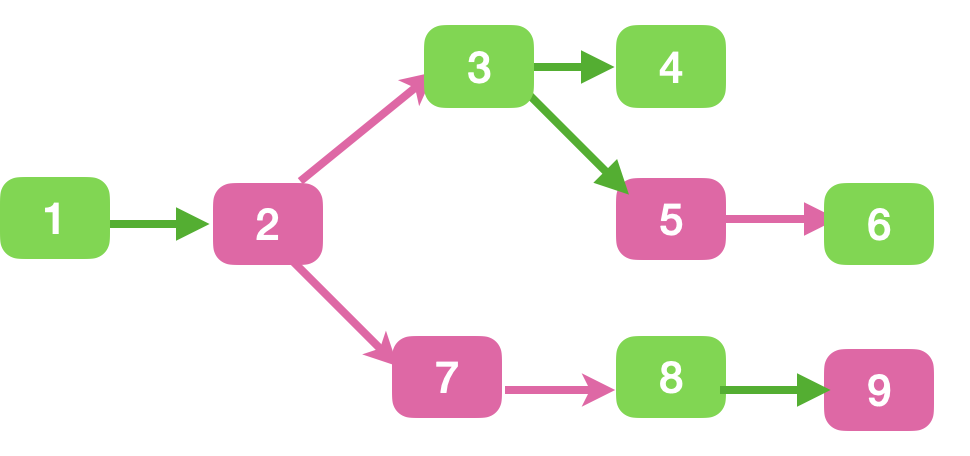
\includegraphics[width=\linewidth]{diagrams/heap.png}
} 
&
\resizebox{5cm}{!}{
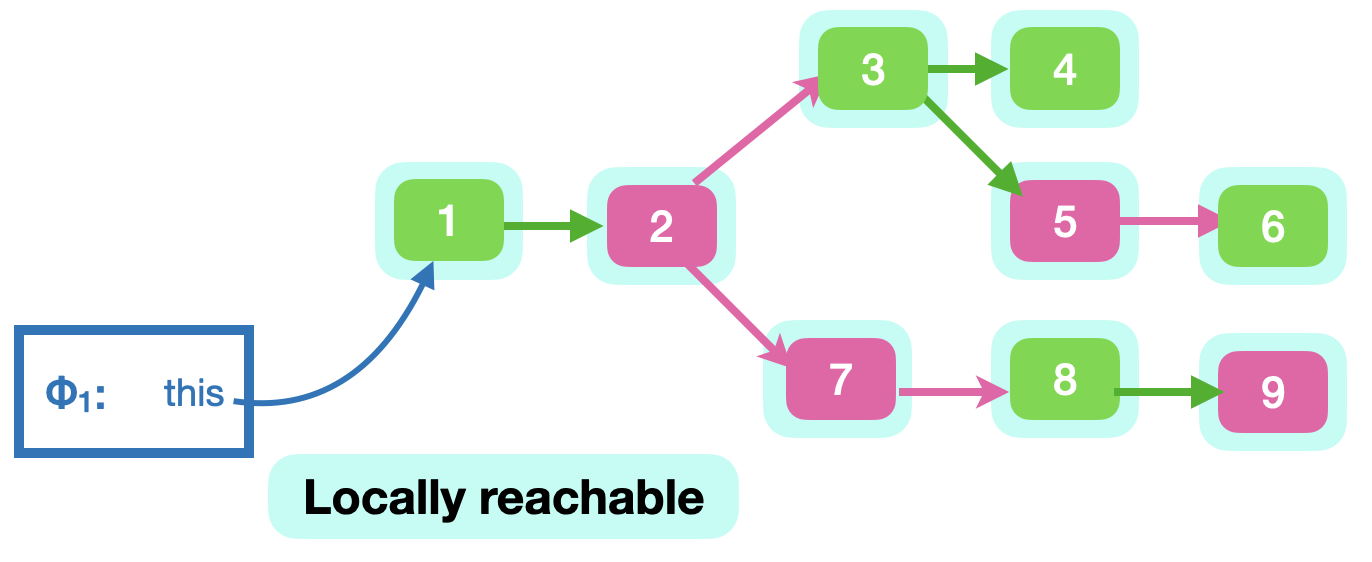
\includegraphics[width=\linewidth]{diagrams/locReachA.png}
} 
&
\resizebox{5cm}{!}{
\includegraphics[width=\linewidth]{diagrams//locReachb.png}
} 
\\
\hline
 a heap
&
Locally Reachable from $\phi_1$
&
Locally Reachable from $\phi_2$
\\
\hline \hline
\end{tabular}
   \caption{A heap, and Locally Reachable Objects. % from $\phi_1$ and $\phi_2$. 
   The distinction of objects into  green or pink is explained in later chapters}
   \label{fig:LReachable}
 \end{figure}

We illustrate these concepts in Fig. \ref{fig:LReachable}: In the middle pane the top frame is $\phi_1$ which maps \prg{this} to $o_1$; all objects are locally reachable. 
In the right pane the top frame is $\phi_2$, which maps \prg{this} to $o_3$, and $x$ to $o_7$; now $o_1$ and $o_2$ are no longer locally reachable.

Lemma  \ref{lemma:relevant} % describes properties of global reachability. 
says that  (\ref{oneGR}) Locally reachable objects are globally reachable. 
(\ref{twoGR}) 
% Any object which will be globally reachable at some future state  and which exists object in the current state, is globally reachable the current state: that is, 
Globally unreachable objects may not become reachable in the future.
\footnoteSD{cite "only connectivity begets connectivity"}
(\ref{threeLR}) A pre-existing object, locally reachable after any number of bounded execution steps, was locally reachable at the first step.


\begin{lemma}
\label{lemma:relevant}
For all module sets $\Mtwo$, states $\sigma$, $\sigma'$,   address $\alpha$, and $\overline \alpha$:
%\footnoteSD{{TODO decide whether $o$ or $\alpha$}}
%and  variables ${\overline z}$, and statements $s:$
\begin{enumerate}
\item
\label{oneGR}
$ \LRelevant \alpha \sigma\ \ \Longrightarrow \ \   \GRelevant \alpha \sigma$
\item
\label{twoGR}
${\leadstoOrigStar {\Mtwo}  {\sigma}  {\sigma'}} \ \ \wedge \ \  \GRelevant \alpha {\sigma'} \ \ \wedge\ \  {\alpha\in \sigma} \ \ \ \Longrightarrow \ \  \ \GRelevant \alpha {\sigma}$.
\item
\label{threeLR}
${\leadstoBoundedStar {\Mtwo}  {\sigma}    {\sigma'}} \ \ \wedge \ \   \LRelevant \alpha {\sigma'}\  \ \wedge\ \  {\alpha\in \sigma} \ \ \ \Longrightarrow \ \ \ \LRelevant \alpha {\sigma}$.
\end{enumerate}
\end{lemma}

{Consider Fig.  \ref{fig:UpSemantics}. %, and Fig.  \ref{fig:UpSemanticsBounded}.
Lemma \ref{lemma:relevant}.\ref{threeLR}  promises that any objects locally reachable in $\sigma_{14}$ which already existed in $\sigma_{8}$, were locally reachable in $\sigma_{8}$. However, the lemma is only  applicable to bounded execution, and as 
$\notLeadstoBoundedStar {\Mtwo} {\sigma_8}  {\sigma_{17}}$, 
the lemma does not promise that  objects locally reachable in $\sigma_{17}$ which already existed in $\sigma_{8}$, were locally accessible in $\sigma_{8}$ -- namely it could be that objects are made globally reachable upon method return, during the step from $\sigma_{14}$ to $\sigma_{15}$.}

 \subsection{\red{EVEN NEWER:} Method Calls and Returns}

 
\sdN{
Calls , and in particular external calls, are a central consideration of our work; therefore a characterization of the states resulting immediately from a method call or a method return is crucial. 
% which a method is called or returned from is important.
 The set ${\_} \triangledown {\_}$ does exactly that:
 }
 
 \sdN{
\begin{definition}
\label{def:push:frame}
Given a state $\sigma$, addresses $\overline \alpha$, and variables or addresses $\overline \va$, we define
\begin{itemize}
\item
$ \PushS  {\alpha} {\sigma} \ =\ \{ \ \sigma' \ \mid\ \exists \phi,\psi,\chi,\phi_n,\phi',\ s.t\ $\\
$\strut \hspace{2.3cm}  \sigma=(\phi\!\cdot\!\psi, \chi)\  \wedge\  \sigma'=(\phi_n\!\cdot\!\phi'\!\!\cdot\!\psi, \chi) \ \wedge\   rng(\phi)=rng(\phi') \ \wedge\ rng(\phi_n)=\overline \alpha \ \   \ \}$
\item
{$ \PushS  {\va}  {\sigma}$ is short for  $ \PushS  {\interpret {\sigma} {\va}} {\sigma} $.}
\end{itemize}
 \end{definition}
}\footnote{\red{DO we also need that $\overline \alpha$ were locally reachable in $\sigma$?}}

\sdN{
%Thus, if $\sigma_a$ is the result of pushing a frame onto $\sigma_b$, then $\sigma_a\in   \PushS  {\alpha} {\sigma_b}$. 
%\sdN{Similarly, if $\sigma_b$ is the result of popping a frame from $\sigma_a$, then $\sigma_a\in   \PushS  {\alpha} {\sigma_b}$.}
 % below Therefore, as 
 Lemma \ref{lemma:push} says that % $\pushSymbol$ characterizes  calls and returns. 
\  (\ref{pushOne}):\  If $\leadstoOrig {\Mtwo} {\sigma}   {\sigma'} $ and $\sigma'\!\in\!\PushS   {\alpha} {\sigma}$ then $\sigma'$ is a  \emph{callee} state of $\sigma$ --  {a direct successor state of    $\sigma$  after calling a method}. % with receiver and arguments $\overline \alpha$). 
 (\ref{pushTwo}):\  If $\leadstoOrig {\Mtwo} {\sigma}   {\sigma'} $ and $\sigma\! \in\! \PushS   {\alpha} {\sigma'}$  then $\sigma'$ is a  \emph{caller} state  of $\sigma$ -- {a direct successor  of $\sigma$}  after returning from a method.
  Also, (\ref{oneLR}):\ A locally reachable object  \sdN{right after entering a call} was also locally reachable before \sdN{entering} the call.
%\kjx{pretty sure we need one other case: (3a) a locally reachable
%  obbject after a call could have been newly created by that call
%  --
%  \red{SD: Thank you for the comment. 
%  (3) is supposed to talk about immediately after entering the call. It was missing an assumption -- in blue. 
%  Please check the text and the maths.}}
}
  
\begin{lemma}% [$\pushSymbol$  for calls and returns]
\label{lemma:push}
For all states $\sigma$, $\sigma'$, modules $\Mtwo$, and addresses $\overline \alpha$. If \ $\leadstoOrig {\Mtwo} {\sigma}   {\sigma'} $, \ then 
\begin{enumerate}
\item
\label{pushOne}
$\sigma'\in   \PushS  {\alpha} {\sigma}  \ \ \Longleftrightarrow \ \ 
\exists x, m.[\ \ \sigma.\prg{cont} \txteq x:=\alpha_0.m(\alpha_1,...\alpha_n); \_\ \ ] $
\item
\label{pushTwo}
$\sigma\in   \PushS  {\alpha} {\sigma'}  \ \ \Longleftrightarrow \ \ \exists x, \alpha'.[\ \  \sigma.\prg{cont}\txteq\alpha' \ \ \wedge \ \ \sigma'.\prg{cont}\txteq x:=\alpha';\_ \ \ ] $
\item
\label{oneLR}
{$\sdN{\leadstoOrig  {\Mtwo}  {\sigma}  {\sigma'}} \ \ \wedge\ \  \sigma'\in \PushS {\alpha} {\sigma}  \ \ \wedge \ \  \LRelevant {\overline \alpha} {\sigma} \ \ \wedge\ \   \LRelevant \alpha {\sigma'} \ \ \ \Longrightarrow$
\\
$\strut \hspace{2cm} \LRelevant \alpha {\sigma}$
}

\end{enumerate}

\end{lemma}

 
\sdN{
 {Consider Fig. \ref{fig:UpSemantics} again: $\sigma_8\!\in\!   \PushS  {\alpha} {\sigma_7}$ for some $\overline \alpha$ -- {thus $\sigma_8$ is a callee state for 
 $\sigma_7$}. Also, 
 $\sigma_{14}\!\in\!\PushS  {\alpha'} {\sigma_{15}}$ for some $\overline {\alpha'}$ -- {thus $\sigma_{15}$ is a caller state for 
 $\sigma_{14}$}.
\footnote{ $\overline \alpha$ may differ from $\overline {\alpha'}$, because between $\sigma_8$ and $\sigma_{15}$ there may 
 have been assignments to local variables.} % -- only the receiver will have remained the same.
}
}
 
% \subsection{\sdN{\red{NEW:} Method Calls and Returns -- Alternative Definition}}
%
% 
%Calls , and in particular external calls, are a central consideration of our work; therefore a characterization of the states resulting immediately from a method call or a method return is crucial. 
%% which a method is called or returned from is important.
% The set ${\_} \triangledown {\_}$ does exactly that:
% 
% 
%\sdN{\begin{definition}
%\label{def:push:frame}
%For state $\sigma$, addresses $\overline \alpha$, and variables or addresses $\overline \va$, we define
%\begin{itemize}
%\item
%$ \PushS  {\alpha} {\sigma} \ \triangleq\ \{ \ \sigma' \ \mid\  \exists \Mtwo, m, \mbox{such that}$\\
%$\strut \ \hspace{2.7cm}  \leadstoOrig {\Mtwo} {\sigma}   {\sigma'}  \ \wedge\  \sigma.\prg{cont} \txteq x:=\alpha_1.m(\alpha_2,...\alpha_n); \_\ \wedge\  {\overline \alpha}=\alpha_1,...\alpha_n \ $\\
%$\strut \ \hspace{2.7cm} \vee$\\
%$\strut \ \hspace{2.7cm}  \leadstoOrig {\Mtwo} {\sigma'}   {\sigma}  \ \wedge\  \exists \alpha',\phi.[\ \sigma'.\prg{cont} \txteq \alpha'  \ \wedge\ \sigma=(\phi\cdot\_,\_) \wedge rng(\phi)=\overline \alpha\ ]\ \   \}$ 
%\item
% {$ \PushS  {\va}  {\sigma}$ is short for  $ \PushS  {\interpret {\sigma} {\va}} {\sigma} $.}
% \end{itemize}
%\end{definition}
%}
%
%% The set $ \PushS  {\alpha} {\sigma}$ characterizes calls as well as returns: 
%Thus, $\sigma_a\in   \PushS  {\alpha} {\sigma_b}$ means that $\sigma_a$ is the result of pushing a frame onto \sdN{$\sigma_b$'s stack}, \red{or} that  $\sigma_b$ is the result of popping a frame from \sdN{$\sigma_a$'s stack}.
% {Consider Fig. \ref{fig:UpSemantics} again:} $\sigma_8\!\in\!   \PushS  {\alpha} {\sigma_7}$ for some $\overline \alpha$ -- {thus $\sigma_8$ is a callee state for 
% $\sigma_7$}. Also, 
% $\sigma_{14}\!\in\!\PushS  {\alpha'} {\sigma_{15}}$ for some $\overline {\alpha'}$ -- {thus $\sigma_{15}$ is a caller state for 
% $\sigma_{14}$}.
%% 
%% Namely, $\sigma_8$ is the first state right after calling a method with receiver and
%% arguments $\overline \alpha$ and $\sigma_{14}$ is the last state before returning from that method call back to $\sigma_{15}$.
%Note that $\overline \alpha$ may differ from $\overline {\alpha'}$, because between $\sigma_8$ and $\sigma_{15}$ there may 
%have been assignments to local variables. % -- only the receiver will have remained the same.
%% Similarly, 
%%  $\sigma_{10}\in\PushS  {\alpha''} {\sigma_9}$ for some $\overline \alpha''$, and  $\sigma_{12}\in\PushS  {\alpha'''} {\sigma_13}$ for some $\overline \alpha'''$, etc.
% 
%
%\subsection{\red{OLD:} Method Calls and Returns}
%
%\susan{I think what I find confusing is that you keep talking about $\sigma$s as if they are stacks whereas $\psi$ is $\sigma$'s stack.
%\red{I am thinking about this. But I do not see where  I talk of  $\sigma$s as if they are stacks; is it where I say "the stack of $\sigma$ " -- would $\sigma$'a stack" be better?}}
%
%{External calls are a central consideration of our work, therefore  the point at which a method is called or returned from is important.
%The operator $\pushSymbol$ describes both call and return:
%% pushing a new frame on the stack: 
% $ \PushS  {\alpha} {\sigma} $ is  the set of states obtained by pushing onto the stack of $\sigma$ a new frame with some continuation  and a local variable map {whose domain has the same cardinality as $\overline \alpha$ and whose range is} $\overline \alpha$, while leaving the heap unmodified.
%The elements of $ \PushS  {\alpha} {\sigma} $ only differ in the identifiers in the local variable map, as well as the continuation  of the top frame. 
%}
%\susan{I think you need a sentence explanation why your frame has suddenly turned into being called $\overline \alpha$. Also given that it is a map why is it important to tell me the size of the domain?\red{Why say that? the text says "a new frame with some continuation  and a local variable map {whose domain has the same cardinality as $\overline \alpha$ and whose range is} $\overline \alpha$", so the fame is not $\overline \alpha$. \sdN{Trying to find better explanation}}}
%
%\begin{definition}
%\label{def:push:frame}
%Given a state $\sigma$, addresses $\overline \alpha$, and variables or addresses $\overline \va$, we define
%\begin{itemize}
%\item
%$ \PushS  {\alpha} {\sigma} \ =\ \{ \ \sigma' \ \mid\ \sigma=(\psi, \chi)\  \wedge\  \sigma'=(\phi\cdot \psi', \chi) \ \wedge\ {\psi\sim\psi'} \ \wedge\ rng(\phi)=\overline \alpha \ \ \mbox{ for some } \phi, \psi, \psi', \chi \ \}$
%\item
%{$ \PushS  {\va}  {\sigma}$ is short for  $ \PushS  {\interpret {\sigma} {\va}} {\sigma} $.}
%\end{itemize}
%{where}
%\\
%{$\strut\ \ \ \  \ \ \ \ \   \psi\sim\psi'$ iff $\psi=\phi_1\cdot\psi_0 \ \wedge \psi=\phi_2\cdot\psi_0\ \wedge \phi_1.\prg{local\_map}=\phi_2.\prg{local\_map}$ for some $\phi_1,\phi2,\psi_0$.}
%
%\end{definition}
%
%{Popping is the counterpart of pushing: $\sigma_a\in   \PushS  {\alpha} {\sigma_b}$ means that $\sigma_a$ is the result of pushing a frame onto $\sigma_b$, and also that  $\sigma_b$ is the result of popping a frame from $\sigma_a$.
% % below 
%Therefore, as  Lemma \ref{lemma:push} says says,  $\pushSymbol$ characterizes  calls and returns.}
%\  (\ref{pushOne}):\  If $\leadstoOrig {\Mtwo} {\sigma}   {\sigma'} $ and $\sigma'\!\in\!\PushS   {\alpha} {\sigma}$ then $\sigma'$ is a  \emph{callee} state of $\sigma$ --  {a direct \emph{successor} state of    $\sigma$ \emph{after} calling a method}. % with receiver and arguments $\overline \alpha$). 
% (\ref{pushTwo}):\  If $\leadstoOrig {\Mtwo} {\sigma}   {\sigma'} $ and $\sigma\! \in\! \PushS   {\alpha} {\sigma'}$  then $\sigma$ is a  \emph{caller} state  of $\sigma'$ -- {a direct \emph{predecessor} of $\sigma'$} \emph{before} returning from a method.
%  
%\begin{lemma}% [$\pushSymbol$  for calls and returns]
%\label{lemma:push}
%For all states $\sigma$, $\sigma'$, modules $\Mtwo$, and addresses $\overline \alpha$. If \ $\leadstoOrig {\Mtwo} {\sigma}   {\sigma'} $, \ then 
%\begin{enumerate}
%\item
%\label{pushOne}
%$\sigma'\in   \PushS  {\alpha} {\sigma}  \ \ \Longleftrightarrow \ \ 
%\exists x, m, \overline{y}.[\ \ \sigma.\prg{cont} \txteq x:=y_0.m(y_1,...y_n); \_\ \ \wedge \ \
%{\overline { \interpret  \sigma y}} = \overline \alpha \ ] $
%\item
%\label{pushTwo}
%$\sigma\in   \PushS  {\alpha} {\sigma'}  \ \ \Longleftrightarrow \ \ \exists x, \alpha'.[\ \  \sigma.\prg{cont}\txteq\alpha' \ \ \wedge \ \ \sigma'.\prg{cont}\txteq x:=\alpha';\_ \ \ ] $
%\end{enumerate}
%
%\end{lemma}
%
% 
%
% {Consider Fig. \ref{fig:UpSemantics} again: $\sigma_8\!\in\!   \PushS  {\alpha} {\sigma_7}$ for some $\overline \alpha$ -- {thus $\sigma_8$ is a callee state for 
% $\sigma_7$}. Also, 
% $\sigma_{14}\!\in\!\PushS  {\alpha'} {\sigma_{15}}$ for some $\overline {\alpha'}$ -- {thus $\sigma_{15}$ is a caller state for 
% $\sigma_{14}$}.
%% 
%% Namely, $\sigma_8$ is the first state right after calling a method with receiver and
%% arguments $\overline \alpha$ and $\sigma_{14}$ is the last state before returning from that method call back to $\sigma_{15}$.
%Note that $\overline \alpha$ may differ from $\overline {\alpha'}$, because between $\sigma_8$ and $\sigma_{15}$ there may 
%have been assignments to local variables. % -- only the receiver will have remained the same.
%% Similarly, 
%%  $\sigma_{10}\in\PushS  {\alpha''} {\sigma_9}$ for some $\overline \alpha''$, and  $\sigma_{12}\in\PushS  {\alpha'''} {\sigma_13}$ for some $\overline \alpha'''$, etc.
%}
%
% \kjx{this magic with $\bigtriangledown$ seems a bit\ldots  magical? \red{SD: magical means "definition unclear"? "motivation unclear"?}
%   why do it this way? \red{SD: what way? Another suggestion?} and we expand on an example here?  \red{SD: I do not understand. Are you asking for an illustrative example?} or is this
%   a standard approach somewhere? \red{SD: I do not know of this concept at other places}}
   


